\documentclass[tikz,border=2pt]{standalone}
\usepackage{amsmath}
\usepackage{pgfplots}
\pgfplotsset{compat=1.18}
\usetikzlibrary{arrows.meta}
\begin{document}
% Exponential log-likelihood for the exact losses 20, 30, 100 (n = 3, sum 150):
% l(lambda) = 3 log lambda - 150 lambda is concave with a zero derivative at lambda-hat = 3/150 = 0.02.
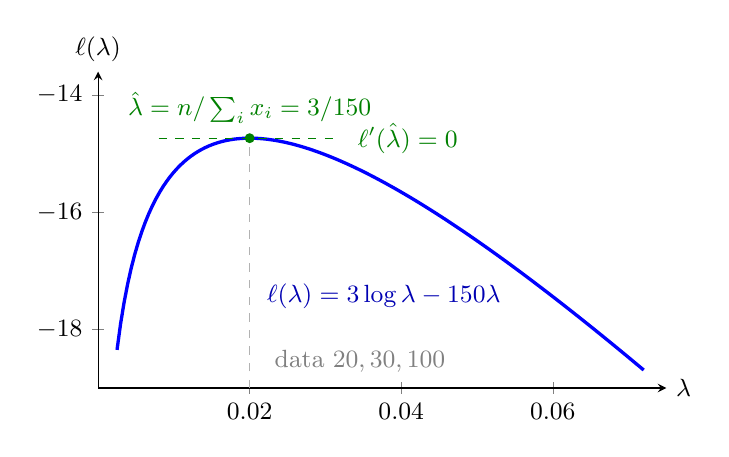
\begin{tikzpicture}[font=\small, >={Latex[length=2mm]}]
  \begin{axis}[
    axis lines=left, xmin=0, xmax=0.075, ymin=-19, ymax=-13.6,
    xtick={0.02,0.04,0.06}, xticklabels={$0.02$,$0.04$,$0.06$}, ytick={-18,-16,-14},
    scaled x ticks=false,
    xlabel={$\lambda$}, ylabel={$\ell(\lambda)$},
    xlabel style={at={(axis description cs:1,0)}, anchor=west},
    ylabel style={rotate=-90, at={(axis description cs:0,1)}, anchor=south},
    samples=150, width=8.8cm, height=5.6cm, clip=false]
    \addplot[blue, very thick, domain=0.0025:0.072] {3*ln(x)-150*x};
    \draw[green!50!black, thin, dashed] (axis cs:0.008,-14.737) -- (axis cs:0.032,-14.737);
    \draw[gray!60, thin, dashed] (axis cs:0.02,-19) -- (axis cs:0.02,-14.737);
    \fill[green!50!black] (axis cs:0.02,-14.737) circle (1.8pt);
    \node[green!50!black, anchor=south] at (axis cs:0.02,-14.65) {$\hat\lambda=n/\textstyle\sum_i x_i=3/150$};
    \node[green!50!black, anchor=west] at (axis cs:0.033,-14.737) {$\ell'(\hat\lambda)=0$};
    \node[blue!70!black, anchor=north west] at (axis cs:0.021,-17.05) {$\ell(\lambda)=3\log\lambda-150\lambda$};
    \node[gray, anchor=south west] at (axis cs:0.022,-18.9) {data $20,30,100$};
  \end{axis}
\end{tikzpicture}
\end{document}
